%
% main.tex -- Paper zum Thema <cahnhilliard>
%
% (c) 2020 Autor, OST Ostschweizer Fachhochschule
%
% TODO: change back to ../../buch.tex
% !TEX root = ../../standalone.tex
% !TEX encoding = UTF-8
%
\newcommand{\di}[2][]{\,\dd[#1]{#2}}
\newcommand{\deriv}[3][]{\frac{\dd[#1]{#2}}{\dd[]{#3^{#1}}}}
\newcommand{\pderiv}[3][]{\frac{\partial^{#1} #2}{\partial #3^{#1}}}
\newcommand{\energy}{\mathcal{E}}
\newcommand{\flux}{{\vec{\jmath}}}

\chapter{Cahn-Hilliard-Gleichung\label{chapter:cahnhilliard}}
\kopflinks{Cahn-Hilliard-Gleichung}
\begin{refsection}
\chapterauthor{Patrik Müller}

Das alltägliche Phänomen,
dass sich eine sorgfältig zubereitete Salatsauce
nach kurzer Zeit wieder in ihre Bestandteile trennt,
ist vielen vertraut.
Trotz intensiven Rührens und Schüttelns scheint es unvermeidlich,
dass das Öl an die Oberfläche steigt,
während der Essig sich am Boden sammelt.
Diese scheinbar einfache Beobachtung offenbart ein faszinierendes physikalisches Phänomen,
das tiefgreifende mathematische und thermodynamische Prinzipien widerspiegelt.

Die Tendenz von Essig und Öl,
sich zu trennen,
lässt sich durch das Konzept der Phasentrennung erklären,
ein Prozess,
der in vielen binären Gemischen beobachtet wird.
Im Zentrum dieses Phänomens steht die Cahn-Hilliard-Gleichung,
die ursprünglich entwickelt wurde,
um die Dynamik der Phasenumwandlung in festen Lösungen und Legierungen zu beschreiben.

In diesem Kapitel werden wir erläutern,
wie sich die Cahn-Hilliard-Gleichung aus einem Variationsprinzip ableiten lässt.
Anschließend analysieren wir die Gleichungen,
um Lösungsansätze für die Herstellung stabilerer Salatsaucen zu entwickeln.

%
% einleitung.tex -- Beispiel-File für die Einleitung
%
% (c) 2024 Patrik Müller, Hochschule Rapperswil
%
% !TeX root = ../../buch.tex
% !TeX encoding = UTF-8
%
\section{Freie Energie\label{cahnhilliard:section:energie}}
\rhead{Freie Energie}

Die freie Energie ist ein grundlegendes Konzept in der Thermodynamik.
Sie beschreibt,
wie viel Energie in einem System verfügbar ist,
um Arbeit zu leisten.
Diese Zustandsgrösse leitet sich aus der inneren Energie,
der Temperatur und der Entropie des Systems ab.
Für ein einfaches,
abgeschlossenes System bei konstanter Temperatur $T$
und konstantem Volumen $V$ wird die Helmholtz-Energie $F$ verwendet.
Sie ist definiert als
\begin{align*}
F
& =
E - TS,
\end{align*}
wobei $E$ die innere Energie und $S$ die Entropie des Systems sind.
Die Helmholtz-Energie ist besonders nützlich in Systemen mit konstantem Volumen,
wie in festen Körpern oder Flüssigkeiten in starren Behältern.
Aus diesem Grund eignet sie sich besonders gut für unser Salatsaucen-Problem.

In den folgenden Abschnitten betrachten wir $F$ als eine gegebene Funktion
für ein homogenes Gemisch zweier Stoffe A und B.
Dabei interessiert uns nur das lokale Mischungsverhältnis der beiden Stoffe,
das wir als
\begin{align*}
c
& =
\frac{N_B}{N_A + N_B}
\end{align*}
definieren.
Dabei bezeichen $N_A$ und $N_B$ die lokale Anzahl der Atome von Stoff A bzw. Stoff B.

\subsection{Freie Energie eines heterogenen Systems}
Um von der gegebenen, inneren Energiefunktion $F(c)$ eines homogenen Systems
auf die innere Energiefunktion $f(c)$ für ein heterogenes System zu gelangen,
kann eine multivariate Taylor-Reihe verwendet werden.
In einem homogenen System ist die Konzentration $c$ überall gleich,
sodass die freie Energie $F(c)$ ausschliesslich von dieser konstanten Konzentration abhängt.
In einem heterogenen System hingegen variiert die Konzentration $c(x)$ räumlich.
Somit ist $f$ abhängig von $\nabla^i c$ für alle $i \in \mathbb{N}$.
Da im homogenen Fall die räumlichen Ableitungen $0$ sind,
wird die Taylor-Reihe um den Punkt
\begin{align*}
\mathbf{c_0}
=
(c, 0, 0, \ldots)
\end{align*}
erstellt.
Somit ergibt sich
\begin{align*}
f(c, \nabla c, \nabla^2 c, \ldots)
=
& F(c)
+ \sum_{i=1}^3 \pderiv{f(\mathbf{c_0})}{c_i} c_i
+ \sum_{i,j=1}^3 \pderiv{f(\mathbf{c_0})}{c_{ij}} c_{ij}
+ \frac{1}{2} \sum_{i,j=1}^3 \frac{\partial^2 f(\mathbf{c_0})}{%
\partial c_i \partial c_j} c_{i} c_{j}
+ \ldots
,
\end{align*}
wobei gilt
\begin{align*}
\quad
c_i
=
\pderiv{c}{x_i}
,\quad
c_{ij}
=
\frac{\partial^2 c}{\partial x_i \partial x_j}
.
\end{align*}
Um den Ausdruck weiter zu vereinfachen,
nehmen wir an,
dass die Materialeigenschaften unseres Gemisches isotrop sind.
Isotropie bedeutet,
dass die Eigenschaften des Materials unabhängig von der Richtung sind,
das heisst,
das Material verhält sich in alle Richtungen gleich.
Dies vereinfacht die Analyse,
da die Einflüsse der räumlichen Ableitungen der Konzentration
in alle Richtungen gleich sein müssen.
Insbesondere bedeutet dies,
dass $f$ gegenüber Spiegelungen ($x_i \rightarrow -x_i$) und
Permutationen ($x_i \rightarrow x_j)$ invariant sein muss.
Aus diesen Eigenschaften lässt sich erkennen,
dass
\begin{align*}
\pderiv{f(\mathbf{c_0})}{c_i}
&=
0,
\\
\pderiv{f(\mathbf{c_0})}{c_{ij}}
&=
\frac{\partial^2 f(\mathbf{c_0})}{\partial c_i \partial c_j}
=
0
\quad \forall i \neq j,
\\
\pderiv{f(\mathbf{c_0})}{c_{ii}}
&=
\kappa_1,
\\
 \pderiv[2]{f(\mathbf{c_0})}{c_i}
&=
\kappa_2
.
\end{align*}
Damit können wir nun die totale innere Energie unseres Systems ausdrücken als
\begin{align}
\mathcal{E}(c)
=
&N_V \int_\Omega f\di{x}
=
N_V \int_\Omega \left[
F(c) + \kappa_1 \Delta c + \frac{\kappa_2}{2} \abs{\nabla c}^2  + \ldots
\right]\di{x}
\label{cahnhilliard:energylong}
,
\end{align}
dabei bezeichnet $N_V$ die Anzahl Moleküle im Gebiet $\Omega$.

\subsubsection{Energieausdruck in angenehmere Form bringen}
Auf \eqref{cahnhilliard:energylong} könnten wir bereits ein Variationsprinzip anwenden.
Jedoch können wir denn Ausdruck zuerst noch weiter vereinfachen.
Wenden wir partielle Integration auf den Laplace-Term von \eqref{cahnhilliard:energylong} an,
erhalten wir
\begin{align*}
\int_\Omega \kappa_1 \Delta c \di{x}
&=
\int_{\partial\Omega} \kappa_1 \nabla c \cdot n \di{s}
- \int_\Omega \nabla \kappa_1 \cdot \nabla c \di{x}
.
\end{align*}
Das Oberflächenintegral können wir gleich $0$ setzen,
da wir ausschliessen,
dass das Gefäss das Mischverhältnis der Salatsauce beeinflusst.
Somit können wir weiter umformen zu
\begin{align*}
\int_\Omega \kappa_1 \Delta c \di{x}
&=-\int_\Omega \sum_{i=1}^3 \pderiv{\kappa_1}{x_i} \pderiv{c}{x_i} \di{x}
\\
&=-\int_\Omega \sum_{i=1}^3 \pderiv{\kappa_1}{c} \pderiv{c}{x_i} \pderiv{c}{x_i} \di{x}
\\
&=
-\int_\Omega \pderiv{\kappa_1}{c} \abs{\nabla c}^2 \di{x}
.
\end{align*}
Wird der erhaltene Ausdruck in \eqref{cahnhilliard:energylong} eingesetzt,
ergibt sich
\begin{align}
\mathcal{E}(c)
&=
N_V \int_\Omega \biggl[
  F(c) + \underbrace{\left( \frac{\kappa_2}{2} - \pderiv{\kappa_1}{c} \right)}_{\frac{1}{2}\epsilon^2} \abs{\nabla c}^2  + \ldots
\biggr]\di{x}
\nonumber
\\
&=
N_V \int_\Omega \left[
  F(c) + \frac{\epsilon^2}{2} \abs{\nabla c}^2  + \ldots
\right]\di{x}
,
\label{cahnhilliard:energy}
\end{align}
wobei $\epsilon$ in der Praxis gemäss \cite{cahnhilliard:freeenergy}
und \cite{cahnhilliard:deriv} häufig als konstant angenommen wird.

%
% cahnhillard.tex -- Herleitung der Cahn-Hilliard-Gleichung
%
% (c) 2024 Patrik Müller, Hochschule Rapperswil
%
% !TeX root = ../../buch.tex
% !TeX encoding = UTF-8
% !TeX spellcheck = de_CH
%
\section{Herleitung der Cahn-Hilliard-Gleichung\label{cahnhilliard:section:herleitung}}
\rhead{Herleitung der Cahn-Hilliard-Gleichung}
Mit \eqref{cahnhilliard:energy} haben wir nun einen Ausdruck auf den wir ein Variationsprinzip anwenden können.
In den folgenden Abschnitten werden wir das Variationsproblem aufstellen und
das Resultat an die Kontinuitätsgleichung koppeln.
Daraus werden wir die Cahn-Hilliard-Gleichung erhalten.

\subsection{Anwenden von Euler-Ostrogradsky-Gleichung}
Bevor wir die Euler-Ostrogradsky-Gleichung anwenden,
entfernen wir den Skalierungsfaktor $N_V$ aus \eqref{cahnhilliard:energy}.
Wir nehmen zudem an,
dass die Änderungen der Konzentration über Distanzen,
die im Vergleich zum intermolekularen Abstand groß sind,
nur geringfügig sind.
Damit können wir die Abhängigkeiten von höheren Ableitungen vernachlässigen.
Auf dieser Grundlage ergibt sich das Funktional
\begin{align}
I(c)
&=
\int_\Omega L(x, c, \nabla c) \di{x}
\nonumber
\\
&=
\int_\Omega F(c) + \frac{\epsilon^2}{2} \abs{\nabla c}^2 \di{x}.
\end{align}
Berechnen wir nun die Ableitungen des Funktionals nach den Feldvariablen erhalten wir
\begin{align*}
\pderiv{I}{c}
&=
\deriv{F}{c}
\\
\pderiv{I}{(\nabla c)}
&=
% \pderiv{}{(\nabla c)} \frac{\epsilon^2}{2} \abs{\nabla c}^2
% &=
\epsilon^2 \sum_{i=1}^3 \pderiv{c}{x_i}
\\
\pderiv{}{x_i}\pderiv{I}{(\nabla c)}
&=
\epsilon^2 \sum_{i=1}^3 \pderiv[2]{c}{x_i}
=
\epsilon^2 \Delta c
% \pderiv{}{(\nabla c)} \left[
% \sum_{i=1}^3 \left( \pderiv{I}{c_i} \right)
% \right]
% \\
% &&&=
% 2 \sum_{i=1}
.
\end{align*}
Somit können wir nun die Euler-Ostrogradsky-Gleichung anwenden:
\begin{align*}
\frac{\delta I}{\delta c}
&=
\deriv{F}{c} -  \epsilon^2 \Delta c
\equiv
\mu
.
\end{align*}
Der erhaltene Ausdruck $\mu$ wird in der Literatur häufig als
\emph{chemisches Potential} bezeichnet.
Im Gleichgewichtszustand gilt $\mu = 0$.
Wir sind jedoch insbesondere daran interessiert,
wie sich unser Gemisch über die Zeit verhält und entmischt.
Daher betrachten wir im folgenden Abschnitt die Dynamik des Systems,
indem wir die zeitliche Entwicklung der Konzentration
$c$ analysieren.

\subsection{Koppeln mit Kontinuitätsgleichung}
Nachdem wir das chemische Potential $\mu$ bestimmt haben,
welches die treibende Kraft für die Veränderung der Konzentration darstellt,
ist der nächste Schritt,
die zeitliche Entwicklung der Konzentration $c(x,t)$ zu untersuchen.
Diese Entwicklung wird durch die Kontinuitätsgleichung
\eqref{buch:symmetrien:felder:eqn:kontinuitaet} gesteuert,
da die Gesamtmasse der Komponenten in einem abgeschlossenen System konstant bleiben muss.
Für das Salatsaucen-Problem gelten folgende Differentialgleichung mit Randbedingungen:
\begin{align}
\begin{aligned}
\pderiv{c}{t}
&=
- \nabla \cdot \flux
,\quad&
x &\in \Omega
\\
\nabla c \cdot n
&=
0
,&
x &\in \partial\Omega
\\
\flux \cdot n
&=
0
,&
x &\in \partial\Omega
.
\end{aligned}
\label{cahnhilliard:continuity}
\end{align}
Nun stellt sich die allerdings die Frage,
was der Fluss $\flux$ in unserem Problem genau sein könnte?
Eine mögliche Inspiration bietet die Wärmeleitungsgleichung,
wo der Fluss proportional zum Gradienten des Temperaturfeldes ist.
Dies führt uns zu der Hypothese, dass auch in unserem Fall der Fluss
durch den Gradienten eines Potentials bestimmt wird.
Daher vermuten wir:
\begin{align*}
\flux
=
- M \nabla \mu
,\quad\text{wobei } M > 0
.
\end{align*}
In der Literatur wird $M$ als die Mobilitätsfunktion bezeichnet,
die häufig als konstant angenommen wird.
Der negative Vorzeichen in der Flussgleichung impliziert,
dass die Bewegung der Teilchen in Richtung des abnehmenden chemischen Potentials erfolgt,
um die freie Energie des Systems zu minimieren.

Im folgenden Abschnitt werden wir untersuchen,
ob der vermutete Fluss $\flux$ wirklich die freie Energie minimiert.
Dies wird es uns ermöglichen,
die Konsistenz unseres Modells zu bestätigen und
die Dynamik der Entmischung in der Salatsauce präzise zu beschreiben.

\subsubsection{Beweis der Energieminimierung}
Da es sich bei unserem Problem um ein Variationsproblem handelt,
sollte die freie Energie minimiert werden.
Dies bedeutet, dass die zeitliche Ableitung des Funktionals  $I$
nicht positiv sein sollte:
\begin{align*}
\deriv{}{t} I
&\leq
0
.
\end{align*}
Mit diesem Ausdruck lässt sich jedoch noch keine Aussage treffen,
ob die Bedingung der Energieminimierung erfüllt wird.
Um den Ausdruck zu vereinfachen,
integrieren wir den zweiten Term partiell und führen einige Umformungen durch.
Dann ergibt sich:
\begin{align*}
\deriv{}{t} I
&=
\int_\Omega \deriv{F}{c} \pderiv{c}{t} + \epsilon^2 \nabla c \cdot \nabla \pderiv{c}{t} \di{x}
.
\end{align*}
Um den Ausdruck weiter zu vereinfach integrieren wir den 2. Term partiell
und wenden noch einige Umformungen an.
Dann resultiert:
\begin{align*}
\deriv{}{t} I
&=
\int_\Omega \deriv{F}{c} \pderiv{c}{t} - \epsilon^2 \Delta c \pderiv{c}{t} \di{x}
+ \int_{\partial\Omega} \epsilon^2 \pderiv{c}{t} \underbrace{\nabla c\cdot n}_{=0} \di{s}
\\
&=
\int_\Omega \mu \pderiv{c}{t} \di{x}
\\
&=
\int_\Omega \mu \nabla \cdot (M \nabla \mu) \di{x}
.
\end{align*}
Durch erneute partielle Integration erhalten wir
\begin{align*}
\deriv{}{t} I
&=
\int_{\partial\Omega} \mu M \nabla \mu \cdot n \di{s} - \int_\Omega \nabla \mu \cdot (M \nabla \mu) \di{x}
.
\end{align*}
Gemäss der Randbedingungen von \eqref{cahnhilliard:continuity}
verschwindet das Oberflächenintegral.
Final erhalten wir also
\begin{align*}
\deriv{}{t} I
&=
-\int_\Omega M \abs{\nabla \mu}^2 \di{x}
\end{align*}
wobei alle Terme im Integral positiv sind.
Somit haben wir bewiesen,
dass unser vermuteter Fluss alle Bedingungen erfüllt.

\subsubsection{Cahn-Hilliard-Gleichung}
Nun haben wir also endlich alle Zutaten zusammen,
um die Cahn-Hilliard-Gleichung aufzustellen:
\begin{align}
\begin{aligned}
\pderiv{c}{t}
&=
\nabla \cdot (M \nabla \mu)
,\quad&
x &\in \Omega
\\
\mu
&=
\deriv{F}{c} -  \epsilon^2 \Delta c
,&
x &\in \Omega
\\
\nabla c \cdot n
&=
0
,&
x &\in \partial\Omega
\\
M \nabla \mu \cdot n
&=
0
,&
x &\in \partial\Omega
\end{aligned}
\label{cahnhilliard:cheq}
\end{align}
Die Cahn-Hilliard-Gleichung beschreibt somit
die zeitliche Entwicklung der Konzentration $c(x,t)$
in Abhängigkeit vom chemischen Potential $\mu$,
und stellt sicher,
dass die freie Energie des Systems minimiert wird,
während die Massenerhaltung gewährleistet ist.

%
% spinodal.tex -- Spinodale Entmischung
%
% (c) 2024 Patrik Müller, Hochschule Rapperswil
%
% !TeX root = ../../buch.tex
% !TeX encoding = UTF-8
% !TeX spellcheck = de_CH
%

\section{Spinodale Entmischung\label{cahnhilliard:section:spinodal}}
\rhead{Spinodale Entmischung}

Nachdem wir die Cahn-Hilliard-Gleichung hergeleitet haben,
möchten wir nun überprüfen,
ob \eqref{cahnhilliard:cheq} tatsächlich das Verhalten von Essig und Öl widerspiegelt.
Zu diesem Zweck wurde eine Simulation mit der Finite-Elemente-Methode (FEM) durchgeführt.
In der Simulation wurden die folgenden Parameter,
Funktionen und Anfangsbedingungen verwendet:
\begin{align*}
\begin{aligned}
M
&=
1,
&
\epsilon
&=
0.01,
&
F(c)
&=
100 c^2 (c - 1)^2,
&
c(x,0)
&=
\frac{2}{3} + 0.01 X
,\; \text{wobei }
X
\sim
\mathcal{U}(-1,1)
.
\end{aligned}
\end{align*}
Dabei stellt $\mathcal{U}(-1,1)$ eine Gleichverteilung von $-1$ bis $1$ dar.
Für $c(x,0)$ wurde absichtlich das aus Kochbüchern typische Verhältnis von
2 Teile Öl zu 1 Teil Essig gewählt.
Wir nehmen ausserdem an, dass die Sauce initial sehr gut gemischt ist.
Der Code für die Simulation ist unter \cite{cahnhilliard:repo} abgelegt.

In Abbildung~\ref{cahnhilliard:fig:chsim} sind die Resultate der Simulation
zu verschiedenen Zeitpunkten dargestellt.
Man kann sehen,
wie sich das homogene Gemisch in seine einzelnen Komponenten zerlegt
und dabei eine Konfiguration
mit möglichst kleiner Grenzoberfläche zwischen den Phasen bildet.
Diese Simulation zeigt anschaulich die spinodale Entmischung,
bei der kleine Fluktuationen in der Konzentration zu einer Trennung der Phasen führen.

\begin{figure}
\centering
\foreach \n [count=\xi] \i in {0,5,10,15,25,50,80,130,300,1500,70000}{
\subfigure[$t = \i\,\tau$]{
\includegraphics[width=0.3\textwidth]{papers/cahnhilliard/presentation/images/ch_sim/\i.pdf}
}}
\subfigure[Farbskala]{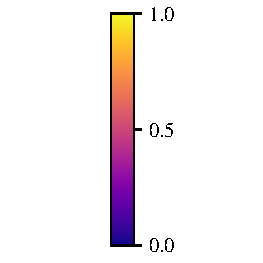
\includegraphics[width=0.3\textwidth]{papers/cahnhilliard/presentation/images/colorbar.book.pdf}}
\caption[Simulation der Cahn-Hilliard-Gleichung]{%
Simulation der Cahn-Hilliard-Gleichung über einen langen Zeitraum.}
\label{cahnhilliard:fig:chsim}
\end{figure}

\subsection{Ursache für die Entmischung}

Die Phasentrennung in einem Gemisch wie Essig und Öl
ist ein faszinierendes physikalisches Phänomen,
das auf die grundlegenden Prinzipien der Thermodynamik zurückgeht.
Um zu verstehen,
warum sich zwei Flüssigkeiten wie Essig und Öl nicht mischen,
müssen wir die Konzepte der freien Energie und
der chemischen Potenziale näher betrachten.

In einem binären Gemisch wird die Gesamtenergie des Systems
durch die freie Energie $F(c)$ bestimmt,
die sowohl die inneren Wechselwirkungen der Moleküle
als auch die Entropie des Systems berücksichtigt.
Diese Funktion reflektiert die energetischen Kosten der Mischung der beiden Komponenten.
Die freie Energie für ein solches Gemisch kann laut \cite{cahnhilliard:deriv}
folgendermassen ausgedrückt werden:
\begin{align*}
F(c)
&=
\omega c (1 - c) + R T \left[ (1-c) \log(1-c) + c \log(c) \right].
\end{align*}
Hierbei ist $\omega$ ein Parameter,
der die Wechselwirkungsenergie zwischen den Komponenten beschreibt,
$R$ die universelle Gaskonstante und
$T$ die Temperatur.

Ein wesentlicher Aspekt ist die unterschiedliche chemische Affinität
der Moleküle zueinander.
Essig,
der hauptsächlich aus Wasser besteht,
und Öl haben sehr unterschiedliche molekulare Strukturen und Wechselwirkungen.
Wasser ist ein polares Molekül und bildet starke Wasserstoffbrückenbindungen,
während Öl aus unpolaren Kohlenwasserstoffmolekülen besteht,
die keine solchen Bindungen eingehen.
Diese unterschiedlichen Wechselwirkungen führen dazu,
dass die Moleküle von Essig und Öl es vorziehen,
sich jeweils mit ihresgleichen zu umgeben,
anstatt sich miteinander zu vermischen.

\subsubsection{Kritische Temperatur}
Wenn wir die freie Energie $F(c)$ eines homogenen Gemisches analysieren,
stellen wir fest,
dass bei bestimmten Temperaturen die freie Energie eine Form annimmt,
die eine Mischung der Komponenten energetisch ungünstig macht.
Insbesondere bei Temperaturen unterhalb einer kritischen Temperatur $T_\text{krit}$
zeigt die freie Energie eine konkave Form im Bereich der mittleren Konzentrationen.
In Abbildung~\ref{cahnhilliard:fig:fc}
ist diese Temperaturabhängigkeit von $F(c)$ dargestellt.
Dies bedeutet,
dass das System energetisch bevorzugt ist,
sich in zwei Phasen mit unterschiedlichen Konzentrationen zu trennen,
um die Gesamtenergie zu minimieren.
Die kritische Temperatur kann durch die Beziehung
\begin{align*}
T_\text{krit}
&=
\frac{\omega}{2 R}
\end{align*}
bestimmt werden.

\begin{figure}
\centering
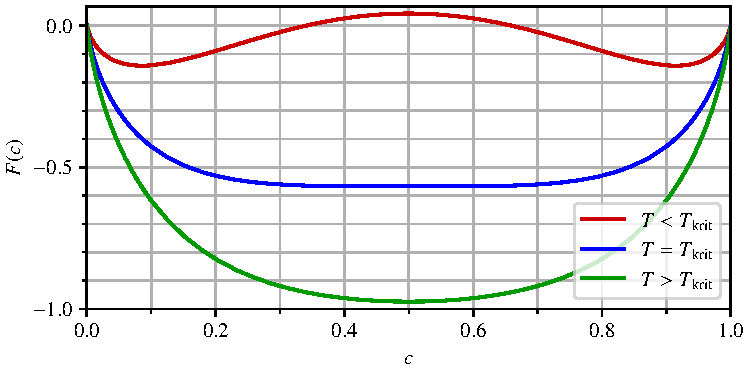
\includegraphics[scale=0.8]{papers/cahnhilliard/presentation/images/energy.book.pdf}
\caption{Temperaturabhängigkeit von $F(c)$}
\label{cahnhilliard:fig:fc}
\end{figure}

Diese Trennung der Phasen wird durch kleine Fluktuationen in der Konzentration initiiert,
die durch thermische Bewegungen der Moleküle verursacht werden.
Sobald diese Fluktuationen auftreten,
führt die minimierte freie Energie dazu,
dass sich die Phasen weiter trennen und stabile Bereiche hoher
und niedriger Konzentration bilden.
Dieser Prozess wird als spinodale Entmischung bezeichnet
und beschreibt die spontane Bildung von Phasen,
die in der Cahn-Hilliard-Gleichung \eqref{cahnhilliard:cheq} modelliert wird.

\subsection{Gegenmassnahmen}
Nachdem wir nun die Ursachen der Phasentrennung verstanden haben,
stellt sich die Frage,
wie man diese Trennung verhindern oder verzögern kann.
Hier sind einige mögliche Gegenmassnahmen:
\begin{enumerate}
\item \emph{Erhöhung der Temperatur:}
Da die Neigung zur Phasentrennung bei höheren Temperaturen abnimmt,
kann eine Erhöhung der Temperatur helfen,
die Mischung stabiler zu halten.
Allerdings ist dies für kalt servierte Salate eher ungeeignet.
\item \emph{Verwendung von Stabilisatoren:}
Stabilisatoren wie Xanthan oder Agar-Agar können der Mischung hinzugefügt werden,
um die Viskosität zu erhöhen und die Bewegung der Tröpfchen zu verlangsamen,
was die Phasentrennung erschwert.
\item \emph{Emulgatoren hinzufügen:}
Emulgatoren sind Moleküle,
die sowohl hydrophile (wasserliebende)
als auch lipophile (fettliebende) Eigenschaften besitzen.
Sie können sich an die Grenzfläche zwischen Essig und Öl anlagern
und die Oberflächenspannung reduzieren.
Dadurch wird die Bildung kleiner,
stabiler Tröpfchen erleichtert,
was die Entmischung verhindert.
Beispiele für Emulgatoren sind Lecithin (in Eigelb enthalten) oder Senf.
\item \emph{Intensives Rühren:}
Mechanisches Rühren oder Schütteln kann die Mischung homogen halten,
indem es die Bildung von Phasengrenzen stört und die Tröpfchen klein hält.
Je intensiver und länger gerührt wird,
desto feiner und stabiler wird die Emulsion.
Allerdings muss dann die Mischung ständig in Bewegung sein,
ansonsten beginnt sofort die spinodale Entmischung.
\end{enumerate}
Zum letzten Punkt möchten wir im folgenden Abschnitt noch zeigen,
dass die Cahn-Hilliard-Gleichung erweitert werden können,
so dass der Einfluss von Rührbewegungen auf die Mischung simuliert werden können.

\subsubsection{Rühren der Mischung}
Da die Cahn-Hilliard-Gleichung ursprünglich für feste Lösungen
und Legierungen entwickelt wurde,
müssen wir sie erweitern,
um auch den Einfluss des mechanischen Rührens in flüssigen Gemischen zu berücksichtigen.
Bis jetzt ist unser Fluss $\flux$ \;nur durch die Diffusion bestimmt,
die durch den Konzentrationsgradienten angetrieben wird.
Das mechanische Rühren erzeugt jedoch eine zusätzliche Flusskomponente,
die ebenfalls berücksichtigt werden muss.
Gemäss \cite{cahnhilliard:deriv-advective} ergibt sich dann
\begin{align}
\begin{aligned}
\pderiv{c}{t} + v \cdot \nabla c
&=
\nabla \cdot (M \nabla \mu)
\\
\mu
&=
\deriv{F}{c} -  \epsilon^2 \Delta c
\\
\nabla \cdot v
&=
0
.
\end{aligned}
\label{cahnhilliard:acheq}
\end{align}
Dabei ist $v$ das durch Rühren erzeugte Geschwindigkeitsfeld.
Nun müssen wir ein geeignetes Geschwindigkeitsfeld finden.
Gemäss \eqref{cahnhilliard:acheq} sollte dieses divergenzfrei sein.
Eine einfache Möglichkeit besteht darin,
die jeweiligen Komponenten des Geschwindigkeitsfeldes
unabhängig von der assoziierten räumlichen Komponente zu machen,
also
\begin{align*}
\begin{aligned}
v_x(x,y,t)
&=
v_x(y,t),
&
v_y(x,y,t)
&=
v_y(x,t)
.
\end{aligned}
\end{align*}
Eine einfache Lösung ist das folgende Geschwindigkeitsfeld:
\begin{alignat*}{2}
v_x(x, y, t)
&=
\alpha \sin(y + \phi_n)
,\quad&
& n \tau \leq t < (n+1) \tau
\\
v_y(x, y, t)
&=
\alpha \sin(x + \psi_n)
,&
& n \tau \leq t < (n+1) \tau
,
\end{alignat*}
wobei die Phasen $\phi_n$ und $\psi_n$ jede Periode zufällig gewählt werden.
Dieses Geschwindigkeitsfeld erzeugt kreisförmige Strömungslinien,
was Rührbewegungen gut abbildet.

\subsubsection{Simulation verschiedener Rührstärken}
Um das Verhalten der Mischung unter unterschiedlichen Bedingungen weiter zu untersuchen,
werden wir \eqref{cahnhilliard:acheq} nun für verschiedene Rührstärken simulieren.
Dazu verwenden wir erneut FEM als Simulationsmethode.
In diesen Simulationen variieren wir die Stärke des Rührens,
repräsentiert durch den Parameter $\alpha$ in unserem Geschwindigkeitsfeld.
So können wir den Einfluss verschiedener Rührintensitäten auf die Phasentrennung
und die Stabilität der Emulsion untersuchen.
Der Code für die Simulation ist unter \cite{cahnhilliard:repo} abgelegt.

In Abbildung~\ref{cahnhilliard:fig:achsim}
sind die Resultate der Simulation mit verschiedenen Rührstärken dargestellt.
Dabei wurden in der Simulation 1000 Zeitschritte berechnet.
In Abbildung~\ref{cahnhilliard:subfig:initial}
ist zudem die Anfangsbedingung $c(x,0)$ ersichtlich.
Diese Ergebnisse verdeutlichen,
wie wichtig die Rührintensität für die Homogenität der Mischung ist.
Eine unzureichende Rührstärke
(wie z.B. in Abbildung~\ref{cahnhilliard:subfig:vweak}
und Abbildung~\ref{cahnhilliard:subfig:weak})
führt dazu,
dass sich die Phasen nur minimal vermischen
und die gewünschte Emulsion nicht erreicht wird.
Bei mittlerer Rührintensität,
wie in Abbildung~\ref{cahnhilliard:subfig:nearly}
beginnt die Mischung sich zu homogenisieren,
aber es sind noch separate Phasen erkennbar.
Erst bei ausreichender Rührstärke wird eine nahezu perfekte Durchmischung erreicht,
die eine stabile Emulsion bildet.
Diese ist in Abbildung~\ref{cahnhilliard:subfig:strong} dargestellt.

Diese Simulationen zeigen deutlich,
dass die richtige Wahl der Rührintensität entscheidend ist,
um eine homogene und stabile Salatsauce herzustellen.
Dies bestätigt,
dass neben den chemischen Eigenschaften der Zutaten auch die mechanischen Einflüsse,
wie das Rühren, eine wesentliche Rolle bei der Herstellung von Emulsionen spielen.

\begin{figure}
\centering
\subfigure[Anfangsbedingung]{

\includegraphics[width=0.3\textwidth]{%
papers/cahnhilliard/presentation/images/ach_sim/initial.pdf}
\label{cahnhilliard:subfig:initial}}
%
\subfigure[$\alpha$ sehr klein]{
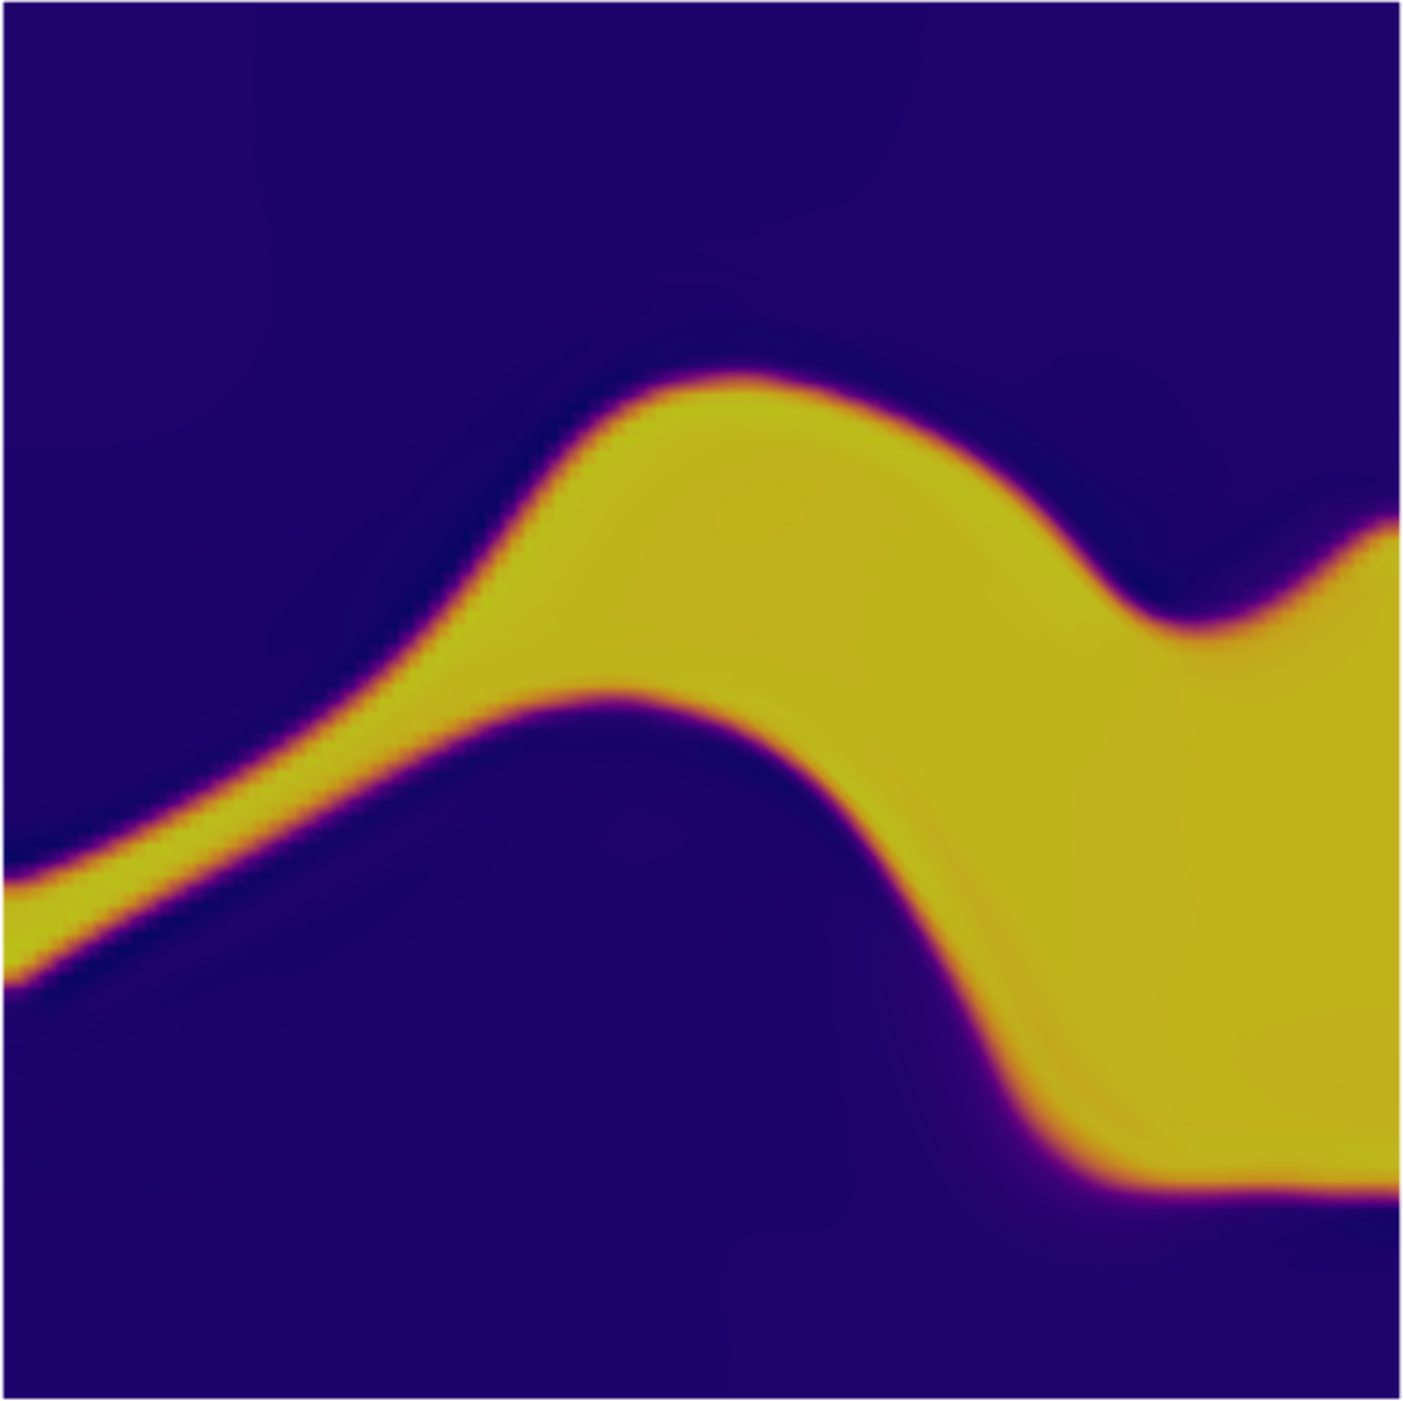
\includegraphics[width=0.3\textwidth]{%
papers/cahnhilliard/presentation/images/ach_sim/very_weak.pdf}
\label{cahnhilliard:subfig:vweak}}
%
\subfigure[$\alpha$ klein]{
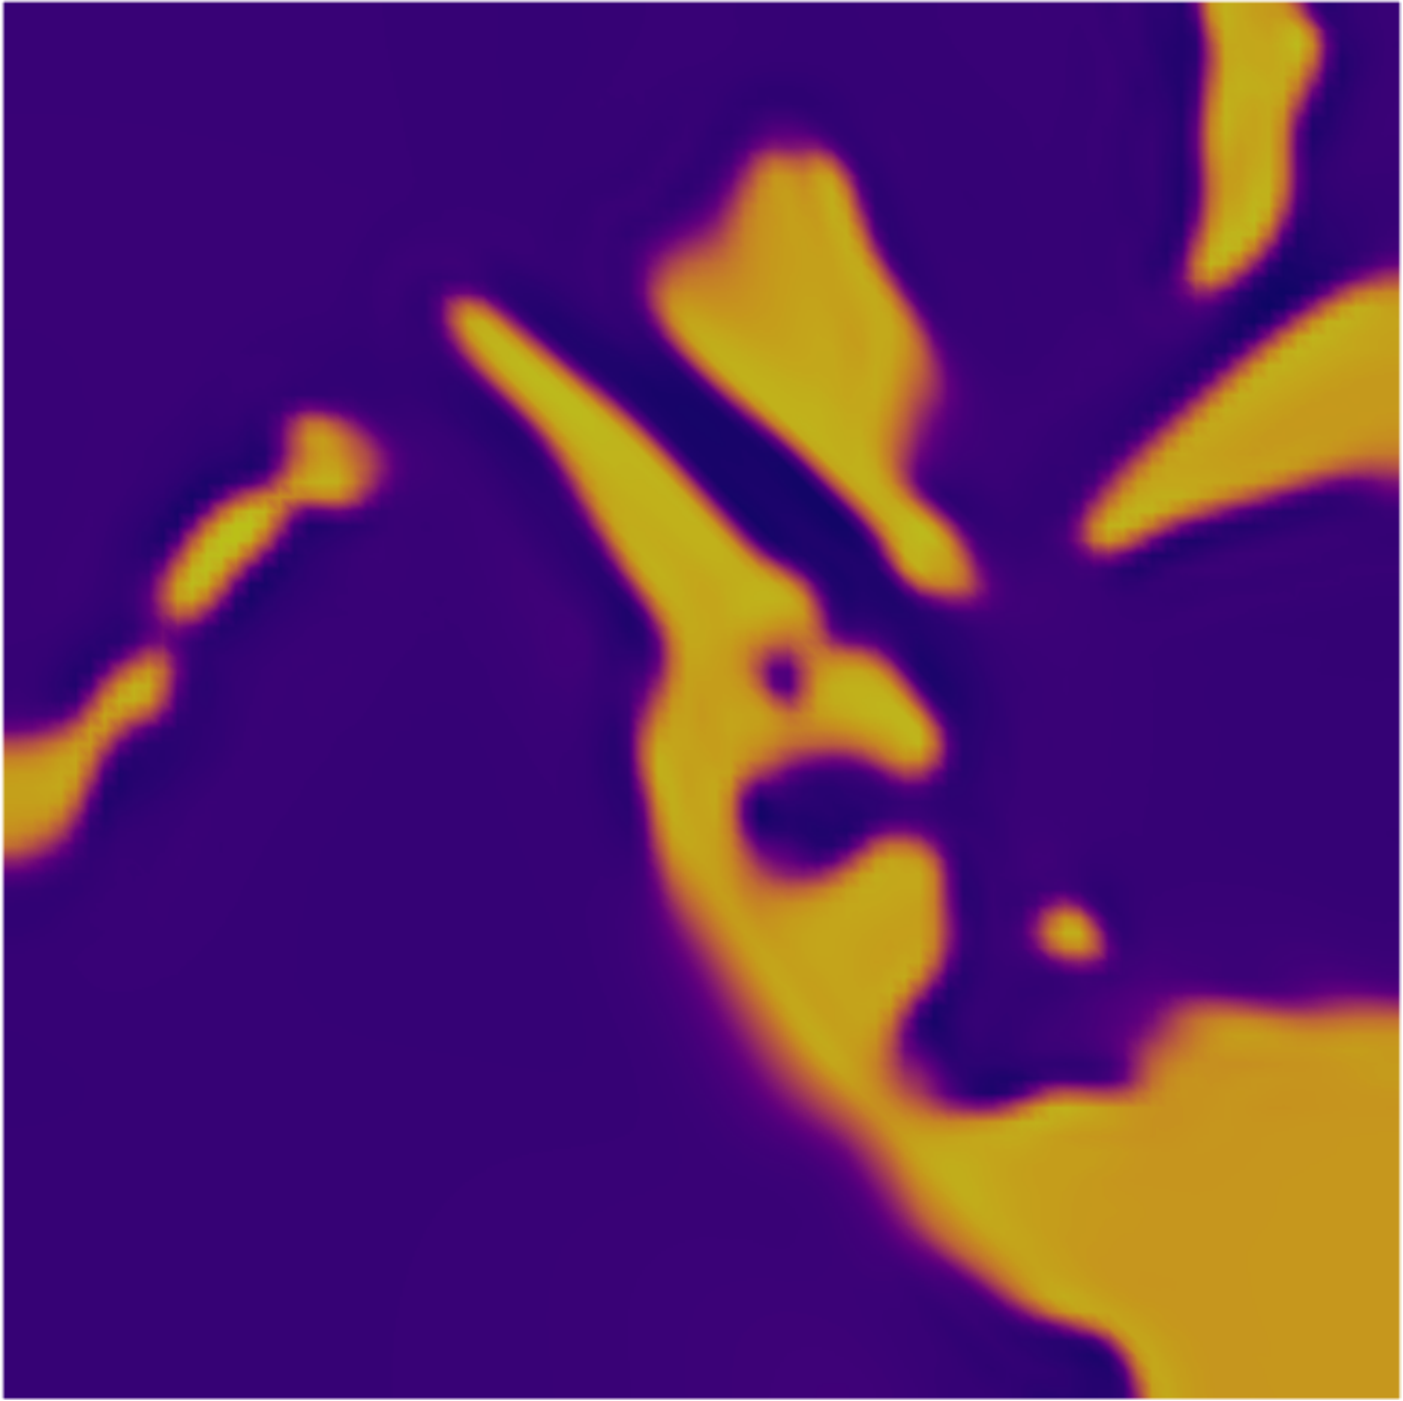
\includegraphics[width=0.3\textwidth]{%
papers/cahnhilliard/presentation/images/ach_sim/weak.pdf}
\label{cahnhilliard:subfig:weak}}
%
\subfigure[$\alpha$ moderat]{
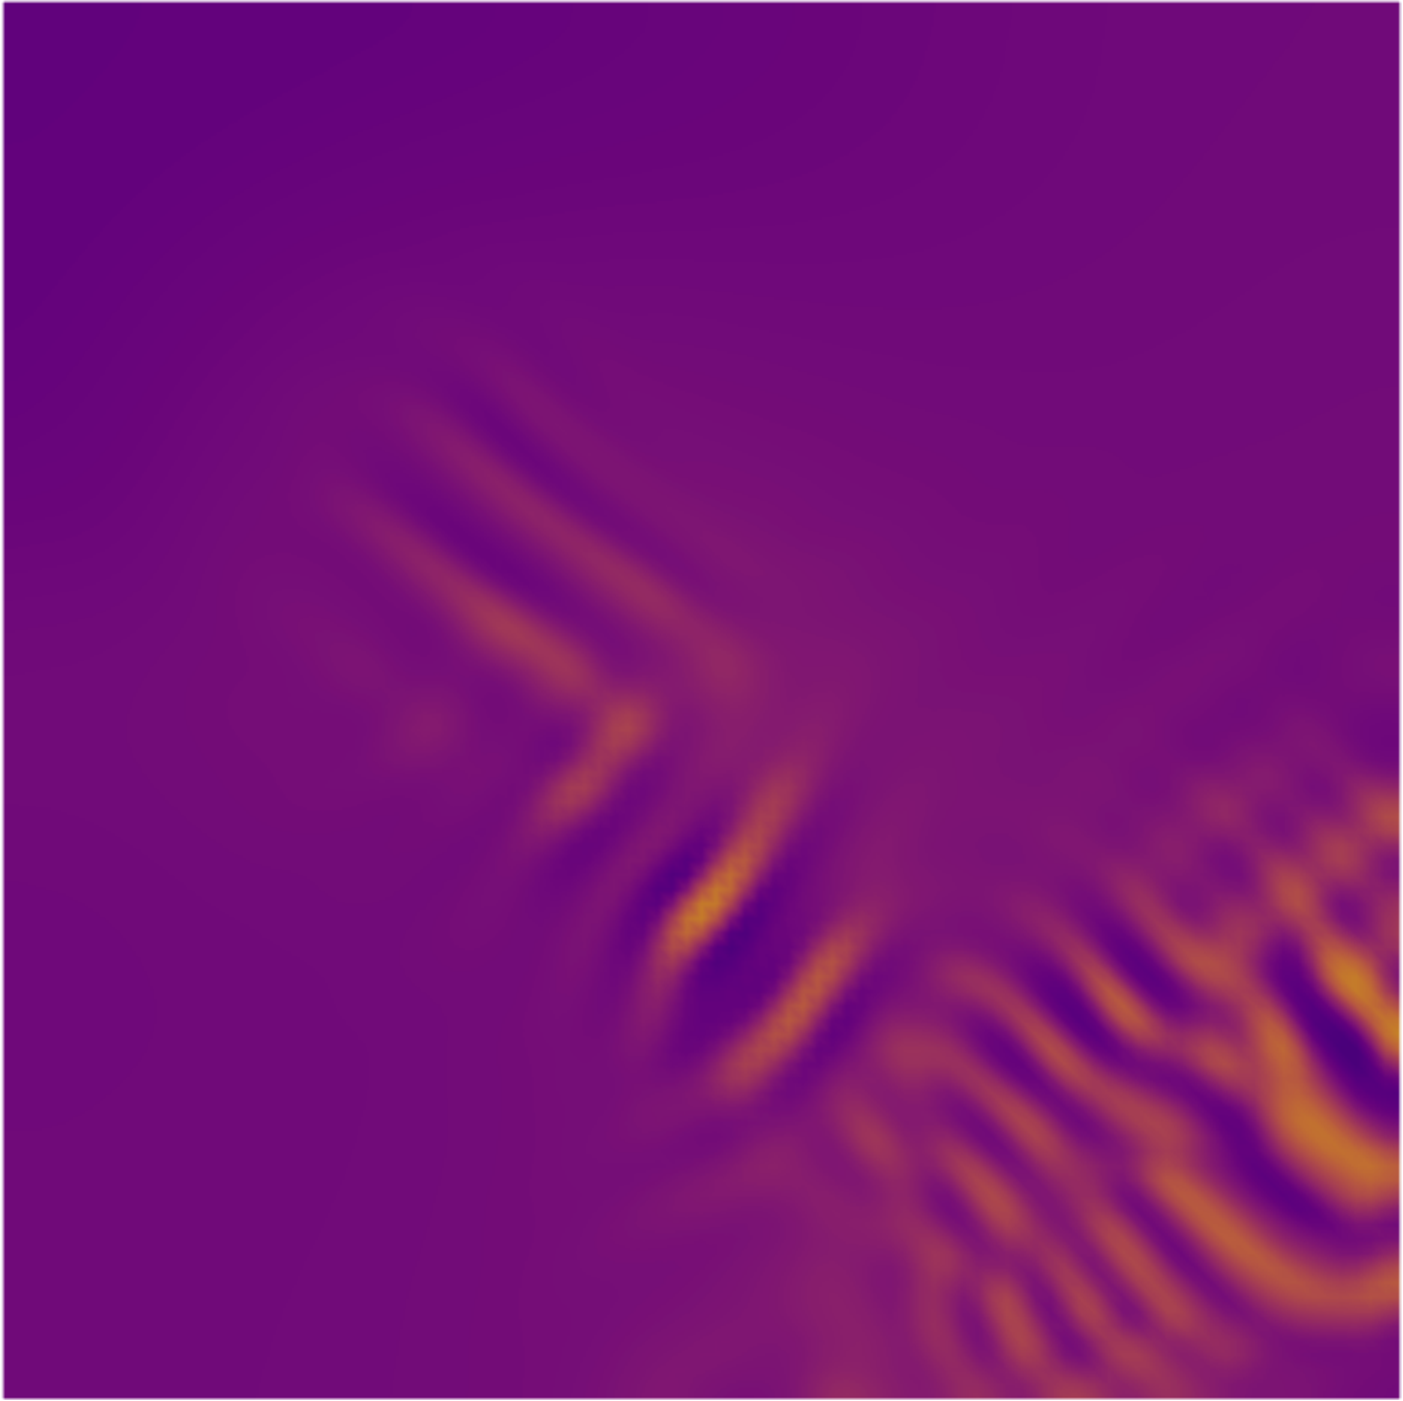
\includegraphics[width=0.3\textwidth]{%
papers/cahnhilliard/presentation/images/ach_sim/nearly.pdf}
\label{cahnhilliard:subfig:nearly}}
%
\subfigure[$\alpha$ gross]{

\includegraphics[width=0.3\textwidth]{%
papers/cahnhilliard/presentation/images/ach_sim/strong.pdf}
\label{cahnhilliard:subfig:strong}}
%
\subfigure[Farbskala]{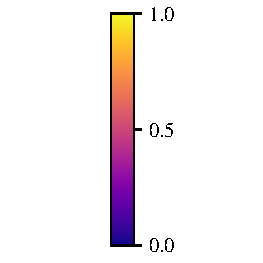
\includegraphics[width=0.3\textwidth]{papers/cahnhilliard/presentation/images/colorbar.book.pdf}}
\caption[Simulation der angepassten Cahn-Hilliard-Gleichung]{%
Anfangsbedingung $c(x,0)$ und
Simulationsresultate von \eqref{cahnhilliard:acheq} nach $1000\,\tau$
mit unterschiedlichen Rührstärken $\alpha$.}
\label{cahnhilliard:fig:achsim}
\end{figure}


\printbibliography[heading=subbibliography]
\end{refsection}
